\chapter{Literature Review}

\section{Cloth Simulation}
The simulation of cloth is a relatively old and well studied field with applications in many different areas, including, but not limited to:
\begin{itemize}
  \item{Virtual Garment Design}
  \item{Virtual Fitting Rooms}
  \item{Films}
  \item{Video Games}
\end{itemize}
Different use cases require different things from the cloth simulation. For example, in virtual garment design, the physical accuracy of the simulation is paramount whereas cloth simulation for video games prioritises real-time simulation, sacrificing accuracy. Hence, many different models for cloth simulation have been proposed.
\\Since this project is concerned with the real-time simulation of cloth, only those models appropriate for real-time simulations have been studied in detail. However, a brief overview of other techniques will be provided. For a more detailed overview of cloth simulation techniques, see \textcite{Ng1996}.

\subsection{Cloth Properties}
Cloth has several properties that should be considered for modelling.

\subsubsection{Mechanical Properties}
Cloth has three mechanical properties that control its behaviour; stretching, shearing and bending, fig. \ref{fig:mechanical properties} shows how each property affects the cloth.
\\Stretching is the displacement of the cloth in either the horizontal or vertical direction. Most cloth has a high resistance to stretching and can typically only be stretched by 10\% \parencites[1]{Yalcn}[4]{Provot2001}.
\\Shearing is the displacement of the cloth in a diagonal direction. Again, most cloths have high shearing resistance and this, coupled with high stretch resistance, makes cloth incompressible.
\\Finally, bending is the overall curvature of the cloth surface. Typically, cloth has low bending resistance and so is easily folded.
\begin{figure}[tp]
   \begin{center}
     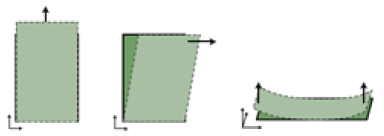
\includegraphics{Figures/mechanical_properties}
   \end{center}
   \caption[Mechanical properties of cloth]{Mechanical properties of cloth \parencite[1]{Yalcn}}
   \label{fig:mechanical properties}
\end{figure}

\subsubsection{Visual Properties}
\label{sec:visual properties}
The mechanical properties of cloth, discussed above, cause cloth to exhibit two visual properties. These properties arise from the fact that cloth is typically non-elastic, due to stretch and shear resistances, but highly flexible, due to low bend resistance.
\\Firstly, cloth will drape over objects and secondly the cloth will form many folds and wrinkles. Fig \ref{fig:visual properties} demonstrates the visual properties of cloth.
\begin{figure}[tp]
   \begin{center}
     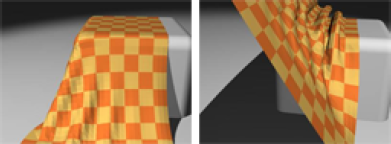
\includegraphics{Figures/visual_properties}
   \end{center}
   \caption[Visual Properties of cloth]{Visual properties of cloth \parencite[1]{Yalcn}}
   \label{fig:visual properties}
\end{figure}

\subsection{Cloth Models}
Techniques for modelling cloth are usually classified as either Geometric or Physically-based, and the choice of which modelling method to use depends on the use-case for the simulation.

\subsubsection{Geometric Models}
This family of techniques were the first models used to simulate cloth. They model the cloth using geometric equations and are especially good at modelling folds and wrinkles.
\\Weil was the first to propose a geometric model in 1986 and uses catenary curves to model the drape and folds of a hanging cloth. Following on from Weil, a number of other geometric models were proposed (see \textcite{Ng1996} for more information).
\\All geometric techniques focus on simulating the appearance of cloth, rather than the physical properties. As such, geometric models are typically more computationally efficient than physically-based models, as there is no need to solve a series of complex equations. However, geometric techniques are unable to accurately simulate the motion of cloth, \parencites[1]{Mongus2012}[2]{Zhang2001}[1-2]{Xinrong2009}, and so are mostly useful for static cloth simulations.
\\As such, geometric models have not been considered for this project.

\subsubsection{Physically-based Models}
By contrast, physically-based models are concerned with the accurate modelling of the physical properties of the cloth and can therefore be used to produce realistic animations.
\\These models typically use a system of partial differential equations (PDE), or other differential equations, to model the cloth. These equations cannot be solved analytically and therefore the system requires discretisation to solve the equations at specific points in space and time. Following discretisation, a physically-based model typically requires the solving of an ordinary differential equation (ODE) of the form \parencite[1]{Baraff1998}:
\begin{equation}
\begin{split}
\label{eq:general ODE}
  &\ddot{x} = M^{-1}\bigg(-\frac{\delta E}{\delta x} + F\bigg)
  \\\text{where:}
  \\&\text{x is a vector representing the geometric state of the system}
  \\&\text{M is a diagonal matrix representing the mass distribution of the system}
  \\&\text{E is a function of x which yields the internal cloth energy}
  \\&\text{F is a function of x and }\dot{x}\text{ which describes other forces}
  \end{split}
\end{equation}
\\Physically-based models can be classified as either Continuum or Discrete.

\paragraph{Continuum Models}\leavevmode\\
Continuum models were the first physical models to be proposed. Techniques in this family model cloth as a continuous surface and utilise continuum mechanics to calculate its behaviour; the Lagrange equations are most commonly used.
\\To discretise the continuous model, a numerical technique, such as a finite element method, is used. This is one of the advantages of continuum methods; they allow the use of a low resolution discretisation without sacrificing the accuracy of the simulation \parencite[4-5]{Wacker2005a}.
\\Another advantage of continuum models are that they are accurate; "they provide accurate models of the material derived directly from mechanical laws and models of material properties" \parencite[200]{Magnenat-Thalmann2006}.
\\This accuracy comes at the cost of computational performance, the main disadvantage of these techniques. The accuracy also renders these models inappropriate for use in dynamic simulations; "the formal and analytical description they require for the mechanical behavior of the material cannot easily be altered to represent transitory and non-linear events. Hence, phenomena such as frequent collisions or other highly variable geometrical constraints cannot be conveniently taken into account" \parencite[200]{Magnenat-Thalmann2006}. 
\\Hence, continuum models are typically only considered appropriate for static simulations, or simulations where accuracy is paramount. As a result, continuum models have not been considered.

\paragraph{Discrete Models}\leavevmode\\
According to \textcite[2]{Choi2002}, "Cloth is not a homogeneous continuum. Therefore modeling fabrics as a continuum and employing FEM or FDM has several potential drawbacks". As a result several discrete, or particle, models have been proposed.
\\With these techniques the discretisation in space is carried out by modelling the cloth as a discrete mesh, either regular or triangular, of point masses, called particles. This sacrifices some of the accuracy of continuum models, as the accuracy will depend on the number of particles used. However, this loss in accuracy is traded off against better computational performance; physical models are the only models that can be used for dynamic, real-time simulations. The discretisation of the cloth has a direct affect on the performance of the simulation; \textcite[5]{Volino2001} have shown that simulation time varies cubically with mesh size. Hence, there is a trade off to be made between accuracy and performance when using discrete models, depending on the use-case.
\\By far the most popular technique is the mass-spring model. This model is popular as it is simple, easy to implement and offers a good balance between accuracy and efficiency. This model is the most common model used for dynamic, real-time simulations and as such, it has been chosen for this project and will now be described in more detail.

\subsection{Mass-Spring Models}
Mass-spring models were first proposed for use in cloth simulation in \textcite{Provot2001}. Using these models, the cloth is discretised as a 2-dimensional mesh of point masses, either regular or triangular, connected by linear springs.

\subsubsection{Provot Model}
Using the mass-spring model proposed in \textcite{Provot2001} the cloth is modelled as a regular mesh of point masses. The points are connected together using three different types of springs:
\begin{itemize}
  \item{Structural springs, connecting particle [i, j] to particles [i + 1, j] and [i, j + 1]. These springs resist structural deformations of the cloth, and provide the overall cloth structure. Structural springs are not enough to provide a realistic cloth model. Fig \ref{fig:structural only} shows the results of running a cloth simulation with structural springs only. As can be seen, this does not produce a realistic image}
  \item{Shear springs, connecting particle [i, j] to particle [i + 1, j + 1] and particle [i + 1, j] to particle [i, j + 1]. These springs provide shearing resistance for the cloth. By adding shear springs, the realism of the model is improved; Fig \ref{fig:structural and shear} shows the improved fidelity afforded by shear springs}
  \item{Bend springs, connecting particle [i, j] to particles [i + 2, j] and [i, j + 2]. These springs model bend resistance}
\end{itemize}

\begin{figure}
\centering
\subfigure[Initial configuration]{\label{fig:structural initial}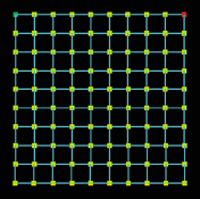
\includegraphics[width=60mm]{Figures/lander_02.png}}
\subfigure[Result of running the simulation]{\label{fig:structural results}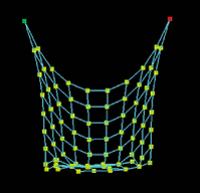
\includegraphics[width=60mm]{Figures/lander_03.png}}
\caption[Cloth with structural springs only]{Cloth with structural springs only \parencite[2]{Lander2000}}
\label{fig:structural only}
\end{figure}

\begin{figure}
\centering
\subfigure[Initial configuration]{\label{fig:shear initial}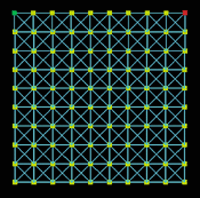
\includegraphics[width=60mm]{Figures/lander_04.png}}
\subfigure[Result of running the simulation]{\label{fig:shear results}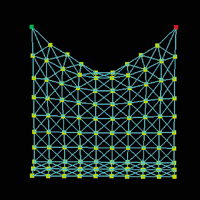
\includegraphics[width=60mm]{Figures/lander_05.png}}
\caption[Cloth with structural and shear springs]{Cloth with structural and shear springs \parencite[2]{Lander2000}}
\label{fig:structural and shear}
\end{figure}

Fig \ref{fig:provot model} shows the arrangement of these springs for a small cloth model.
\begin{figure}[tp]
   \begin{center}
     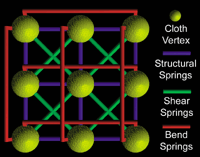
\includegraphics{Figures/provot_mesh_structure.png}
   \end{center}
   \caption[Provot cloth model]{Provot cloth model \parencite[2]{Lander2000}}
   \label{fig:provot model}
\end{figure}

To animate the mesh, forces are applied to the particles and are calculated using Newton's second law:
\begin{equation}
\begin{split}
\label{eq:newton second law}
  &F_{ij} = m_{ij}a_{ij}
\\\text{where:}
\\&F_{ij}\text{ is the total sum of forces acting on particle ij}
\\&m_{ij}\text{ is the mass of particle ij}
\\&a_{ij}\text{ is the acceleration of particle ij}
\end{split}
\end{equation}

The total force acting on a particle is defined as:
\begin{equation}
\label{eq:total force}
  F_{total} = \Sigma F_{external} + \Sigma F_{internal}
\end{equation}

F$_{external}$ are external forces acting on the mesh, such as gravity and wind.
\\Gravity is calculated by:
\begin{equation}
\begin{split}
\label{eq:gravity}
  &F_{g} = m_{ij}G
  \\\text{where:}
  \\&\text{G is the gravitational constant}
\end{split}
\end{equation}
Wind is calculated by:
\begin{equation}
\begin{split}
\label{eq:wind}
  &F_{wind} = w(n_{ij}\bullet\overrightarrow{W})
  \\\text{where:}
  \\&\text{n$_{ij}$ is the surface normal of particle ij}
  \\&\text{$\overrightarrow{W}$ is the wind direction vector}
  \\&\text{w is the wind constant}
\end{split}
\end{equation}

F$_{internal}$ are the resultant forces of the springs connecting the mesh.
\\The spring force is calculated using the Hooke equation \parencite[201]{Parent2012}:
\begin{equation}
\begin{split}
\label{eq:hooke equation}
  &F_{spring} = -k_{s}(L_{c}-L_{r})\frac{p_{2}-p_{1}}{\parallel p_{2}-p_{1}\parallel}
  \\\text{where:}
  \\&\text{k$_{s}$ is the spring stiffness coefficient}
  \\&\text{L$_{c}$ is the current length of the spring}
  \\&\text{L$_{r}$ is the initial, or rest, length of the spring}
  \\&\text{p$_{1}$ \& p$_{2}$ are the positions of the two connected particles}
\end{split}
\end{equation}
Using this equation, the cloth will be modelled with pure elastic springs and will oscillate indefinitely. However, as mentioned in \ref{sec:visual properties} and \textcite[1]{Provot2001}, cloth is a non-elastic medium and therefore the model needs to account for the energy lost due to internal friction in the cloth.
\\This is typically modelled as an extra internal damping force, calculated using \parencite[201]{Parent2012}:
\begin{equation}
\begin{split}
\label{eq:spring damping}
  &F_{damping} = -k_{d}(\dot{p_{2}}-\dot{p_{1}})\bullet\bigg(\frac{p_{2}-p_{1}}{\parallel p_{2}-p_{1}\parallel}\bigg)\bigg(\frac{p_{2}-p_{1}}{\parallel p_{2}-p_{1}\parallel}\bigg)
  \\\text{where:}
  \\&\text{k$_{d}$ is the spring damping coefficient}
  \\&\text{$\dot{p_{1}}$ \& $\dot{p_{2}}$ are the velocities of the two connected particles}
\end{split}
\end{equation}

\subsubsection{Choi Ko Model}
A different mass-spring model was proposed in \textcite{Choi2002} and aims to improve the buckling behaviour of the cloth, resulting in more realistic draping and wrinkling behaviour.
\\The cloth is modelled in a similar way to the Provot method, but additional bend springs are added, connecting particle [i, j] to particle [i + 2, j + 2] and particle [i + 2, j] to particle [i, j + 2]; fig \ref{fig:choi ko model} shows the arrangement of springs.
\begin{figure}[tp]
   \begin{center}
     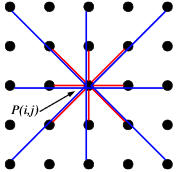
\includegraphics{Figures/choi_ko_model.png}
   \end{center}
   \caption[Choi Ko cloth model]{Choi Ko cloth model \parencite[2]{Choi2002}}
   \label{fig:choi ko model}
\end{figure}
\\This model uses an energy-based approach, of the general formula \ref{eq:general energy equation}\parencite[3]{Bartels2014}, to calculate the forces acting on individual particles.
\begin{equation}
\begin{split}
\label{eq:general energy equation}
  &F = \bigg(\frac{\delta E(S)}{\delta x}, \frac{\delta E(S)}{\delta y}, \frac{\delta E(S)}{\delta z}\bigg)
  \\\text{where:}
  \\&\text{E(S) is an energy function of S, a representation of the cloth's state}
\end{split}
\end{equation}
Two types of interactions are defined, type 1 and type 2. Type 1 interactions model stretch and shear resistances, the red lines in \ref{fig:choi ko model}, and are represented by a linear spring model. Type 2 interactions model bend forces, the blue lines in \ref{fig:choi ko model}, and helps prevent the so called post-buckling instability problem. The interested reader should see \textcite{Choi2002} for more information on the energy functions for each interaction type.

\subsubsection{Justification of Choice}
Mass-spring models are suitable for use in this project as they are efficient and simple to implement; "Mass-spring models are the most efficient as well as the simplest of the cloth models.  This method is one of the most popular techniques for simulating cloth, especially when interactive frame rates are required" \parencite[2]{Zink2007}. As this project is concerned with the real time animation of cloth, mass-spring models are therefore the obvious choice.
\\Mass-spring models are also the most common method of modelling cloth in video games, used in games such as Alan Wake, \parencite[2]{Enqvist2010}, and Hitman: Codename 47, \parencite[1]{Jakobsen2005}, as well as commercial physics engines for games, such as Havok\textsuperscript{\textregistered} and PhysX\textsuperscript{\textregistered}. Again, since this project is concerned with the simulation of cloth for use in a video game, mass-spring models are the logical choice.
\\In particular, the Provot model was used for this project as the force-based approach requires the solving of a much simpler series of equations than the energy-based approach of the Choi Ko model, and is therefore likely to be more computationally efficient.
\\\\One disadvantage of the mass-spring model is that it does not achieve realistic animation of cloth as "mass-spring systems do not model any specific material and are not related to measured properties of real clothes" \parencite[3]{Wacker2005a}. However, by careful tuning of the spring stiffness coefficients pleasing results can be achieved; \textcite{Mongus2012} have shown that, with tuning, mass-spring models can reproduce the drape of a cloth with an accuracy of 97\%.
\\Another disadvantage of mass-spring models is what Provot calls 'super-elasticity'; springs are allowed to deform too much, leading to unrealistic looking cloth. This is caused because "the springs are “ideal” and they have unlimited linear deformation rate" \parencite[3]{Vassilev2001}. To counter this effect, Provot suggests enforcing length constraints on structural and shear springs. First the position of the particles are updated, then the deformation of the springs are calculated. If this deformation value is greater than some threshold, $\tau_{c}$, then the position of the connected particles are adjusted so the deformation rate equals $\tau_{c}$. Fig \ref{fig:super-elasticity} shows the super-elasticity problem and the results of employing Provot's corrective method. As can be seen, correcting the super-elasticity results in a much more realistic model.

\begin{figure}
\centering
\subfigure[Super-elastic effect]{\label{fig:super-elasticity}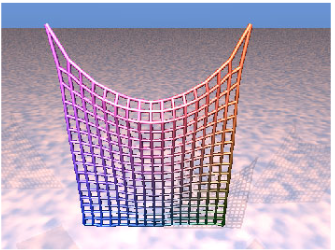
\includegraphics[width=60mm]{Figures/super_elasticity.png}}
\subfigure[Result of correcting super-elasticity]{\label{fig:super-elasticity correction}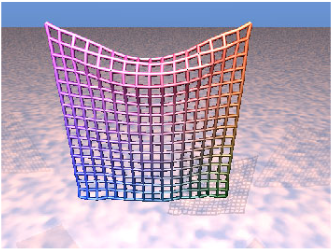
\includegraphics[width=60mm]{Figures/super_elasticity_corrected.png}}
\caption[Super-elasticity problems]{Super-elasticity problems \parencite[4,6]{Provot2001}}
\label{fig:super-elasticity}
\end{figure}

\subsection{Numerical Integration for Mass-Spring Models}
As mentioned above, physically-based models for cloth simulation require solving a series of differential equations, discretised in space and time. According to \textcite[5]{Wacker2005a}, "since particle systems already represent a discretization in space, only a system of ordinary differential equations has to be solved". For the Mass-Spring model using Newtonian mechanics a series of second order ODEs, of the form \ref{eq:newtonian ODE}, must be solved \parencite[5]{Zink2007}.
\begin{equation}
\label{eq:newtonian ODE}
  \frac{\delta^{2}x}{\delta t^{2}} = M^{-1}F(x, v)
\end{equation}
This can be converted into a coupled series of first order ODEs by separating the position and velocity \parencite[5]{Zink2007}:
\begin{equation}
\label{eq:1st order ODE}
  \frac{\delta}{\delta t} \bigg(\begin{array}{c}  x \\ v \end{array}\bigg) = \bigg(\begin{array}{c}  v \\ M^{-1}F(x, v) \end{array}\bigg)
\end{equation}
Equations \ref{eq:newtonian ODE} and \ref{eq:1st order ODE} cannot be solved analytically, and therefore it is necessary to use a numerical method, or integrator, to approximate them at discrete time intervals. There are many integration methods that could be chosen, typically classified as either explicit or implicit, and the most popular choices will be described now.

\subsubsection{Explicit Integrators}
\label{sec:explicit}
Most of the early work on physically-based cloth simulation used explicit integrators as they are simple and easy to implement; they only require information about the state of the system at the previous interval to calculate the current state.
\\The most commonly used explicit integrators are the Runge-Kutta family of integrators.

\paragraph{Euler}\leavevmode\\
The first order Runge-Kutta integrator, or explicit Euler, was used in \textcite{Provot2001} to approximate a Mass-Spring system.
\\Equation \ref{eq:1st order ODE} is approximated by \parencite[3]{Wang2009a}:
\begin{equation}
\begin{split}
\label{eq:explicit euler formal}
  &v_{i + \Delta t} = v_{i} + \Delta t F(t_{i}, v_{i})
  \\\text{where:}
  \\&\text{$v_{i}$ is the velocity of a particle at time interval i}
  \\&\text{$\Delta t$ is the time step}
\end{split}
\end{equation}
When applied to the Provot Mass-Spring model, this gives \parencite[3]{Provot2001}:
\begin{equation}
\begin{split}
\label{eq:explicit euler provot}
  &a_{i, j}(t + \Delta t) = \frac{1}{m_{i, j}}F_{i, j}(t)
  \\&v_{i, j}(t + \Delta t) = v_{i, j}(t) + \Delta ta_{i, j}(t + \Delta t)
  \\&x_{i, j}(t + \Delta t) = x_{i, j}(t) + \Delta tv_{i, j}(t + \Delta t)
  \\\text{where:}
  \\&\text{$a_{i, j}$, $m_{i, j}$, $v_{i, j}$ and $x_{i, j}$ are the acceleration, mass, velocity and position of particle i, j respectively}
\end{split}
\end{equation}
The explicit Euler method is computationally cheap but can result in numerical instability if too large a time step is used. Mathematically, the explicit Euler method is stable only if the time step is less than the natural period of the system, approximated as $\pi\sqrt{\frac{m}{K}}$, where K is the maximum stiffness in the system. \textcite[2]{Vassilev2001} found that in fact explicit Euler is only stable for $\Delta t$ values less than $0.4\pi\sqrt{\frac{m}{K}}$. 
\\As cloth generally does not stretch easily, this results in high stiffness in the structural and shear springs, which necessitates the use of a small time step if the explicit Euler integrator is chosen. This can impact the overall performance of the simulation, as while this integrator is cheap, the frequency of calculations is high as a result of the time step limitations.

\paragraph{Midpoint}\leavevmode\\
The explicit Midpoint integrator is a second order Runge-Kutta method and modifies the Euler integrator to give greater stability.
\\Equation \ref{eq:explicit euler formal} is modified to give the following \parencite[3]{Wang2009a}:
\begin{equation}
\label{eq:midpoint}
  v_{i + \Delta t} = v_{i} + \Delta t F\bigg(t_{i} + \frac{\Delta t}{2}, v_{i} + \frac{\Delta t}{2}F(t_{i}, v_{i})\bigg)
\end{equation}
Since this method requires two derivatives, the computational cost is greater than Euler. However, because the midpoint method affords greater numerical stability (see fig \ref{fig:stability regions}), a larger time step can be used which increases the overall simulation performance; \textcite{Wang2009a} have shown that the midpoint integrator offers close to twice the simulation performance over explicit Euler.
\begin{figure}[tp]
   \begin{center}
     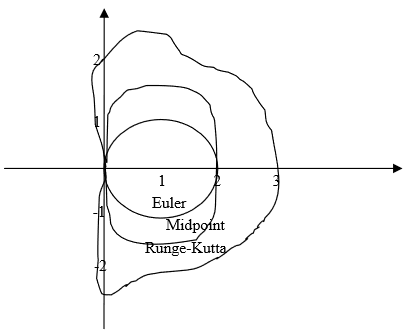
\includegraphics{Figures/stability_diagram.png}
   \end{center}
   \caption[Explicit integrator stability regions]{Explicit integrator stability regions \parencite[4]{Wang2009a}}
   \label{fig:stability regions}
\end{figure}

\paragraph{Fourth order Runge-Kutta}\leavevmode\\
The Fourth order Runge-Kutta integrator offers greater stability using larger time steps over the midpoint method and is formulated as \parencite[3]{Wang2009a}:
\begin{equation}
\begin{split}
\label{eq:4th order rk}
  &v_{i + \Delta t} = v_{i} + \frac{\Delta t}{6}(k_{1} + 2k_{2} + 2k_{3} +  k_{4})
  \\&k_{1} = F(t_{i} + v_{i})
  \\&k_{2} = F\bigg(t_{i} + \frac{\Delta t}{2}, v_{i} + \frac{\Delta t}{2}k_{1}\bigg)
  \\&k_{3} = F\bigg(t_{i} + \frac{\Delta t}{2}, v_{i} + \frac{\Delta t}{2}k_{2}\bigg)
  \\&k_{4} = F\bigg(t_{i} + \Delta t, v_{i} + \frac{\Delta t}{2}k_{3}\bigg)
\end{split}
\end{equation}
This integrator has a significantly higher computational cost than the other methods discussed, however \textcite[4]{Volino2001} have shown that the Runge-Kutta integrator supports time steps almost six times larger than the midpoint method. Therefore, given that Runge-Kutta is three times as computationally expensive as midpoint, this suggests that this integrator can lead to twice the overall simulation performance. \textcite[4]{Wang2009a} have also shown that the fourth order Runge-Kutta integrator offers simulation performance over midpoint and explicit Euler.

\paragraph{Verlet}\leavevmode\\
Verlet integration is an alternative to the Runge-Kutta family of integrators. It avoids velocity calculations by approximating the velocity of a particle using its previous positions.
\\A particle's new position is approximated by \parencite[2]{Mongus2012}:
\begin{equation}
\label{eq:verlet}
  x_{i + \Delta t} = 2x_{i} - x_{i - \Delta t} + a_{i + \Delta t}\Delta t^{2}
\end{equation}
This method is computationally fast and reasonably stable, as "velocity is implicitly given and consequently it is harder for velocity and position to come out of sync" \parencite[1]{Jakobsen2005}. However it does still suffer from time step issues; figures 11 and 13 in \textcite[14-15]{Wacker2005a} show that below a certain threshold Verlet integration is less stable than explicit Euler, but more stable over that threshold.

\subsubsection{Implicit Integrators}
According to \textcite[1]{Baraff1998}, "Explicit methods are ill-suited to solving stiff equations because they require many small steps to stably advance the simulation forward in time". Therefore they propose an implicit integrator for use in cloth simulation since implicit integrators are unconditionally stable regardless of step size. 
\\However implicit integrators are computationally more expensive than their explicit equivalents, as "they involve the resolution of a large and sparse linear equation system for each iteration" \parencite[4]{Volino2005}. Since they are unconditionally stable however, this can be countered by simply using a larger time step. The guaranteed stability of these methods also reduces the accuracy of the simulation, as they introduce inherent numerical damping, which increases as the time step increases (see \textcite[4]{Volino2001}). As such, there is a balance to be found between performance and accuracy of the simulation with implicit integrators.
\\The most common implicit integrator is the implicit, or backward, Euler method which will be described now. It should be noted that there are many other implicit integrators available.

\paragraph{Euler}\leavevmode\\
First proposed for use in cloth simulation in \textcite{Baraff1998}, the implicit, or backward, Euler method is an adaptation of the explicit Euler method.
\\Equation \ref{eq:explicit euler provot} is modified to give \parencite[3]{Kang2000}:
\begin{equation}
\label{eq:implicit euler 1}
  v^{t + \Delta t}_{i} = v^{t}_{i} + F^{t + \Delta t}_{i}\frac{\Delta t}{m_{i}}
\end{equation}
$F^{t + \Delta t}_{i}$ cannot be calculated at the current time step, and so must be approximated as \parencite[3]{Kang2000}:
\begin{equation}
\label{eq:implicit euler 2}
  F^{t + \Delta t} = F^{t} + \frac{\delta F}{\delta x}\Delta x^{t + \Delta t}
\end{equation}
$\Delta x^{t + \Delta t}$ can be written as $\Delta t(v^{t} + \Delta v^{t + \Delta t})$ and so eq. \ref{eq:implicit euler 2} can be rewritten, giving the series of linear equations \parencite[3]{Kang2000}:
\begin{equation}
\begin{split}
\label{eq:implicit euler 3}
  &\bigg(I - \frac{\Delta t^{2}}{m}\frac{\delta F}{\delta x}\bigg)\Delta v^{t + \Delta t} = F^{t}\frac{\Delta t}{m}
  \\&\text{where:}
  \\&\text{I is the identity matrix}
\end{split}
\end{equation}
Thus, implicit Euler involves calculating $\Delta v^{t + \Delta t}$ every iteration using:
\begin{equation}
\label{eq:implicit euler 4}
  \Delta v^{t + \Delta t} = \bigg(I - \frac{\Delta t^{2}}{m}\frac{\delta F}{\delta x}\bigg)^{-1}F^{t}\frac{\Delta t}{m}
\end{equation}
$\frac{\delta F}{\delta x}$ is the negated Hessian matrix, denoted as H, and can be approximated as \parencite[3]{Kang2000}:
\begin{equation}
\begin{split}
\label{eq:implicit euler 5}
&H_{ij} =
  \begin{cases}
    k_{ij}       & \quad \text{if } i \neq j\\
    -\sum_{i \neq j}{k_{ij}}  & \quad \text{if } i = j\\
  \end{cases}
\\&\text{where:}
\\&\text{$k_{ij}$ is the spring stiffness}
\end{split}
\end{equation}
As a result, the implicit Euler method requires the computation of an n x n matrix each iteration, and thus increasing the size of the mesh greatly impacts the performance of this method.
\\However, if the stiffness of the springs and mass of the particles are constant throughout the simulation then $\bigg(I - \frac{\Delta t^{2}}{m}H\bigg)^{-1}$ can be precomputed, giving performance gains.
\\This method has been shown by \textcite{Volino2001} to be stable for any time step value, however as the time step increases, the accuracy decreases rapidly over a certain threshold. Using the method described above, it is also not possible to use an adaptive time step or to vary the mass or stiffness of the model as the cost of computing H every iteration is high. As such, many researchers, such as \textcite{Mesit2007} and \textcite{Kang2000}, have presented faster approximation methods for the implicit Euler integrator.

\subsubsection{Chosen Integration Methods}
Four integrations methods were chosen for investigation by this project.
\begin{itemize}
\item{Explicit Euler. This is the simplest integrator and one of the most popular in the literature but it is also most likely to impact simulation performance due to its reliance on small time steps}
\item{Fourth order Runge-Kutta. Computationally more expensive than explicit Euler, but stable with larger time steps, therefore offering an interesting comparison between computational cost and simulation performance}
\item{Verlet. Chosen as it is an explicit integrator that is not part of the Runge-Kutta family}
\item{Implicit Euler. Unconditionally stable regardless of time step, Chosen to provide a contrast between explicit and implicit integrators}
\end{itemize}